\chapter{Solution}

%Description (comparaison statique dynamique)

Dans l'article \textit{Code Generator Testing in Practice} \cite{sturmer2004}, Stürmer et Conrad donne une approche de réalisation
d'une suite de logiciel permettant de tester convenablement un générateur de code.
Ils considèrent 4 étapes principales pour le test d'un générateur de code. La première étape est la spécification formelle, ils représentent les spécifications
formelles sous forme d'un graphe de règles dans le but de traduire ces règles en cas de tests concrets qui serviront à l'étape suivante ou l'on possède
un simulateur capable de fournir le résultat des tests. On génère ensuite le code à partir du ou des modèles définis auparavent. Il faut ensuite
comparer les résultats de l'éxecution du code compilé avec les résultats attendu.

Leur approche est résumé dans la figure \ref{codegen}.

\begin{figure}
	\label{codegen}
	\centering
	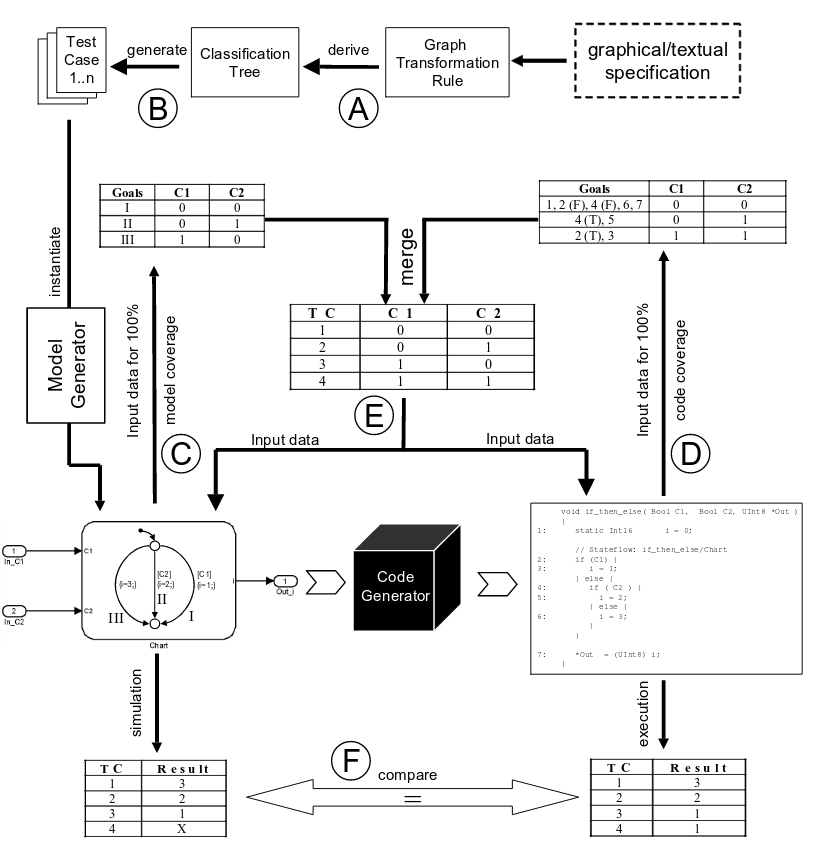
\includegraphics[width=0.7\linewidth]{images/codegen.png}
	\caption{Schéma de l'approche de Sturmer}
\end{figure}

%Principaux points (json)

Cette solution possède le défaut d'être extremmement dépendante du générateur à tester. Pour chaque générateur, il nous faut un oracle complexe
qui saura déterminer la sortie attendu en fonction du modèle. Nous avons voulu réaliser un logiciel de test qui soit facilement adaptable à des
projets différents ayant peu de choses en commun.

C'est pour cela que nous avons choisis de nous focaliser sur les dernières étapes, c'est à dire que
nous avons développer un logiciel qui prend en entrée un fichier contenant les instructions de générations et d'execution du code ainsi que le résultat
attendu en fin d'éxecution. Le but alors est de vérifier que le code généré produit bien le résultat attendu lors de l'éxecution. La partie de génération
des cas de tests est laissé à l'utilisateur de notre logiciel. Cette approche est certes moins strict qu'une analyse statique du programme généré par
le compilateur, comme le fait le compilateur XTend, mais permet d'obtenir des résultats tout aussi interessant.

%Documentation

%Software engineering
